\chapter{Precautions}\label{ch:precautions}

This chapter consolidates the mandatory safety rules that accompany every Digifiz Replica and Digifiz Replica Next instrument cluster. Ignoring any of these items is the fastest way to damage the electronics or obtain unreliable readings.

\begin{enumerate}
    \item \textbf{Disconnect the vehicle battery before starting the installation.} Working on a powered harness feels faster, but several dashboards have already been destroyed by short circuits caused by a live loom.
    \item \textbf{Never feed the sensor inputs with an external voltage source.} The coolant temperature, oil temperature, outside temperature, and fuel level channels are designed for passive sensors only. Even a “harmless” test through a resistor burns the measurement circuitry.
    \item \textbf{Remember that Generation~1 and 1.5 panels have no internal fuse.} The first protective element is the 15~A fuse in the Volkswagen fuse box. It reacts far too late to save the cluster from wiring mistakes.
    \item \textbf{Shield the unit from direct sunlight.} Prolonged exposure washes out the LCD segments and permanently reduces contrast.
    \item \textbf{Do not attempt to overdrive the LED backlight.} Generations~1, 1.5, and~2 use fixed-current lighting. If the daytime image is dim, add shading around the binnacle rather than increasing the drive current.
    \item \textbf{Beware of resonances in cable-driven speedometers.} Mechanical drives often oscillate at 40--60~km/h. Fit the supplied electronic sensor---it ships with all current Gen~1.5 and Gen~2 kits---whenever possible.
    \item \textbf{Plan external MFA controls for Generation~2 dashboards.} The VW badge touch sensor was removed, so MFA mode switching must come from the steering-column stalk or another external switch.
    \item \textbf{Account for the standby current.} A Generation~2 cluster draws roughly 11--13~mA from the vehicle battery even when the ignition is off. This quiescent consumption cannot be reduced.
    \item \textbf{Instantaneous fuel consumption is not factory fitted.} The feature can be retrofitted to Gen~1 and Gen~1.5 units following the instructions at\newline\url{https://www.youtube.com/watch?v=qWqvYc9388U}, but it has not been validated for Gen~2 hardware.
\end{enumerate}

\begin{figure}[htbp]
    \centering
    \begin{subfigure}{0.46\textwidth}
        
\includegraphics[width=\linewidth]{digifiz_manual/image001.jpg}
        \caption{Label emphasising battery disconnection during installation.}
    \end{subfigure}\hfill
    \begin{subfigure}{0.46\textwidth}
        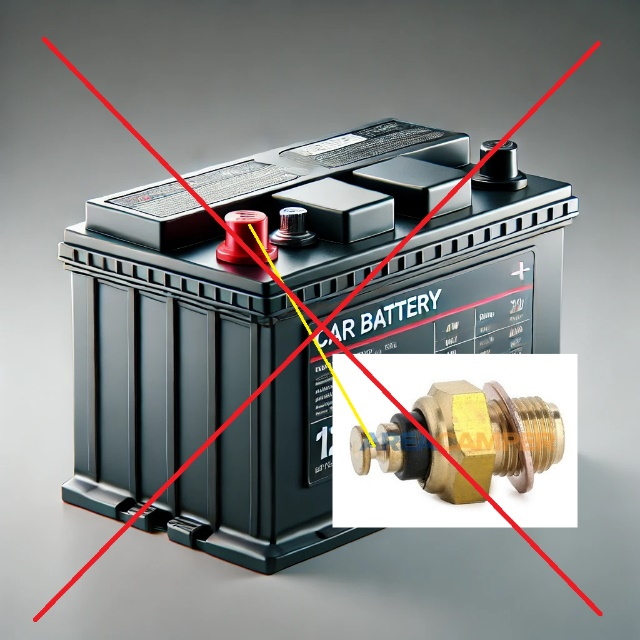
\includegraphics[width=\linewidth]{digifiz_manual/image002.jpg}
        \caption{Warning supplied with the sensor harness against external voltage.}
    \end{subfigure}
    \caption{Safety placards shipped with the wiring kit.}
\end{figure}
